\documentclass[10pt,a4paper]{article}
\usepackage[top=15mm, bottom=15mm, left=18mm, right=18mm]{geometry}
\usepackage[table]{xcolor}
\usepackage{tcolorbox}
\usepackage{tabularx}
\usepackage{booktabs}
\usepackage{multicol}
\usepackage{tikz}
\usetikzlibrary{positioning, arrows.meta, shapes.geometric, calc}
\usepackage{hyperref}
\usepackage{enumitem}
\usepackage{mathpazo}
\usepackage{amsmath}
\usepackage{makecell}
\usepackage{float}
\usepackage{placeins} 

\setlength{\parindent}{0pt}
\setlength{\parskip}{3pt}
\setlist{nosep, itemsep=1pt, parsep=1pt, topsep=2pt}
\raggedbottom

\begin{document}

% ==========================================================================
% PAGE 1: Motivation & Business Case
% ==========================================================================
\begin{center}
    {\LARGE \textbf{\textsf{NeuroLens}}}\\[4pt]
    {\large \textbf{\textsf{\textcolor[HTML]{0284c7}{An Elastic Cloud-Native Neuromarketing SaaS for Video Engagement Prediction}}}}\\[6pt]
    {\footnotesize \textsf{\textcolor[HTML]{64748b}{CS5224 Cloud Computing $\bullet$ Preliminary Project Report $\bullet$ AY 2026/2027}}}\\[4pt]
    {\footnotesize \textsf{\textcolor[HTML]{64748b}{Chan Wei Jie Dylan (E1122343) $\bullet$ Chong Xin Wei (E1122103) $\bullet$ Low Hoa Meng, Kelvin (E1508421) $\bullet$ Lum Zi Yuan Joshua (E0297372) $\bullet$ Tan Zhi Hao Brandon (E1136804)}}}\\[2pt]
    \rule{\textwidth}{0.4pt}
\end{center}
\vspace{2mm}

\section*{\textsf{1. Motivation \& Business Case}}
\subsection*{\textsf{1.1 The Power and Inaccessibility of Neuromarketing}}
Neuromarketing, the application of cognitive neuroscience to decode how the brain responds to advertising, is one of the most direct methods of commercial evaluation. When viewers watch an ad inside an fMRI scanner, second-by-second changes in cortical blood oxygenation capture attentional and emotional responses that traditional self-report methods cannot: they suffer from post-hoc rationalisation, social desirability bias, and memory decay.

Venkatraman et al. (2015) demonstrated that fMRI measures significantly outperformed conventional survey and biometric instruments in predicting real-world advertising sales elasticity. Yet physical fMRI requires multi-million-dollar 3-Tesla scanners and clinical staff, costing \textbf{\$10,000--\$15,000 per commercial}, placing it out of reach for most studios and agencies.

\subsection*{\textsf{1.2 The Modern Catalyst: Faster Production, Harder Evaluation}}
Video advertising is now dominated by fast-scrolling mobile feeds such as TikTok, Instagram Reels, and YouTube Shorts, where viewers can dismiss any video with a swipe. The opening hook matters, but the challenge extends beyond the first few seconds: even a well-hooked viewer can be lost at a jarring transition or a mid-video lull.

Simultaneously, generative AI tools such as Runway, Sora, and CapCut allow creators and marketing teams to produce numerous creative variants rapidly. This creates a \textbf{Production--Evaluation Asymmetry}: generating alternatives is fast and inexpensive, but understanding where and why a creative might lose its audience (at any point in the timeline) before publication remains difficult.

\subsection*{\textsf{1.3 NeuroLens: Pre-Flight Creative Diagnostics}}
NeuroLens addresses this gap with a self-service, pre-flight workflow. Rather than recruiting participants for physical brain scans, it uses Meta's \textbf{TRIBE v2 (d'Ascoli et al., 2026)}, a research model trained to predict average cortical fMRI responses to naturalistic video. The model produces predictions across \textbf{20,484 points on the cortical surface}; NeuroLens makes this output actionable by summarising it into five region-specific activation signals based on atlas-mapped brain regions (Destrieux et al., 2010):
\begin{itemize}
    \item \textbf{Faces (FFA; Kanwisher et al., 1997):} Highlights when faces and spokespeople are strongly represented.
    \item \textbf{Action \& Movement (EBA; Downing et al., 2001):} Highlights bodies, gestures, and physical movement.
    \item \textbf{Scenes \& Settings (PPA; Epstein \& Kanwisher, 1998):} Highlights locations, environments, and changes of setting.
    \item \textbf{Social Interaction (STS; Allison et al., 2000; Frith \& Frith, 2006):} Highlights gaze, human interaction, and social movement.
    \item \textbf{Audio (Binder et al., 2000):} Highlights when dialogue, music, and other sounds are strongly represented. A dual-pass silent baseline comparison isolates where the soundtrack changes the cortical response, letting creators review audio timing and compare alternatives.
\end{itemize}

\textbf{Commercial licensing:} TRIBE v2 is currently released under CC BY-NC 4.0, which does not permit commercial use. Before launching NeuroLens as a commercial service, the project would therefore require either a negotiated commercial licence from Meta or a model whose licence permits commercial deployment. We acknowledge this licensing constraint upfront, but believe the commercial potential and the cloud-architecture challenges it motivates make NeuroLens a worthwhile project for this course regardless of the model's current licence.

\subsection*{\textsf{1.4 Target Audience \& Competitor Matrix}}
NeuroLens targets two audiences: \textit{independent creators} reviewing second-by-second predicted responses to flag underperforming moments for re-editing, and \textit{boutique digital agencies} comparing creative variants before committing client media spend. Competing platforms such as Neurons and Dragonfly AI predict visual attention from video features; NeuroLens instead uses a model trained on measured fMRI data, producing multimodal cortical timelines, billed via a credit-pack and subscription model.

\begin{table}[htbp]
    \centering
    \caption{NeuroLens Competitor Analysis and Cost Comparison}
    \begin{tabularx}{\textwidth}{|X|X|X|X|X|}
    \hline
    \rowcolor{black!5}
    \textbf{Dimension} & \makecell[l]{\textbf{Physical fMRI} \\ \textbf{Study}} & \makecell[l]{\textbf{Webcam Facial-} \\ \textbf{Coding}} & \makecell[l]{\textbf{Predictive} \\ \textbf{Analytics}} & \textbf{NeuroLens} \\
    \hline
    \textbf{Underlying Method} & Measured fMRI & Computer-vision facial analysis & AI-predicted visual attention & \textbf{Predicted fMRI responses} \\
    \hline
    \textbf{Turnaround} & Days to weeks & 3 hours -- 3 days & Seconds to minutes & \textbf{Seconds to minutes} \\
    \hline
    \textbf{Indicative Cost} & \$10,000+ per study & \$850 -- \$4,000 per video & Quote-based pricing & \textbf{\$0.90 per 30s video*} \\
    \hline
    \end{tabularx}
    \vspace{4pt}
    {\raggedright \footnotesize *Effective cost per video within subscription/credit-pack pricing; not billed per transaction.\par}
\end{table}

% ==========================================================================
% PAGE 2: Business Model & Economics
% ==========================================================================
\vspace{-6mm}
\section*{\textsf{2. Business Model \& Economics}}

\subsection*{\textsf{2.1 The Cloud Economic Justification: Converting CAPEX into OPEX}}
TRIBE v2 integrates three frozen feature extractors (LLaMA 3.2-3B, V-JEPA 2-Giant, and Wav2Vec-BERT 2.0) with a cortical readout transformer, totalling $\sim$5B parameters and demanding $\sim$40 GB of active VRAM during full trimodal inference. This comfortably exceeds commodity 16 GB and 24 GB consumer GPUs. Practical on-premise self-hosting therefore requires an enterprise-grade high-memory workstation:
\begin{itemize}
    \item \textbf{The Hardware Penalty:} An enterprise workstation equipped with a 48 GB professional GPU (e.g., NVIDIA RTX 6000 Ada) or high-memory accelerator costs approximately \textbf{\$6,000--\$9,000} upfront, with ongoing power, cooling, and driver maintenance overhead.
    \item \textbf{The Utilisation Problem:} Ad testing is episodic. An agency may run 20 jobs during an intense editing sprint, then nothing for days. An on-premise GPU sits idle over 80\% of the time, inflating the amortised cost per job.
    \item \textbf{The Elastic Cloud Remedy:} Following Armbrust et al. (2010), NeuroLens pools high-performance cloud GPUs on demand. Queue-depth autoscaling scales workers to zero during off-peak periods, with no idle cost.
\end{itemize}

\subsection*{\textsf{2.2 Monetisation Strategy \& Unit Economics}}
We model inference costs on an AWS EC2 \texttt{g6e.2xlarge} Spot instance (single 48 GB NVIDIA L40S GPU, $\sim$\$0.75/hr). On a warm worker, the two-pass analysis of a 30-second ad runs in 28--45 seconds, consuming approximately \textbf{\$0.008 in raw GPU compute}. In practice, cold-start events and idle cooldown periods between jobs raise the blended infrastructure cost to approximately \textbf{\$0.035 per ad}. Factoring in per-request overhead (S3 storage, Aurora writes, ALB traffic) and \textbf{amortised payment gateway fees}, the fully-loaded variable cost is approximately \textbf{\$0.10 per ad}.

To ensure micro-transaction fees do not erode margins, NeuroLens avoids per-analysis billing in favour of a \textbf{credit-pack and monthly subscription model}. Retailing at an average of \textbf{\$0.90 per ad}, the service yields a \textbf{blended gross margin of approximately 89\%}. The fixed platform baseline in \texttt{ap-southeast-1} (ALB, Aurora Serverless v2, CloudWatch) totals approximately \textbf{\$70--\$85/month}, which is comfortably covered at low subscriber volumes.

Crucially, factoring in the fixed platform baseline, elastic cloud hosting breaks even against a single-GPU on-premise workstation ($\sim$\$225/month amortised) at approximately \textbf{1,475 videos/month} (using the \$0.10/video fully-loaded cost). This suggests that for bursty workflows, a scale-to-zero cloud architecture is vastly more capital-efficient than self-hosting.

\subsection*{\textsf{2.3 End-to-End User Journey}}
The five-step workflow is illustrated below: SSO login, direct S3 upload via presigned URL, worker-side duration validation, asynchronous job tracking via polling, and interactive Chart.js visualiser with exportable CSV.

% Locked strictly here with [H] to prevent floating under Section 3
\begin{figure}[H]
    \centering
    \resizebox{\textwidth}{!}{%
    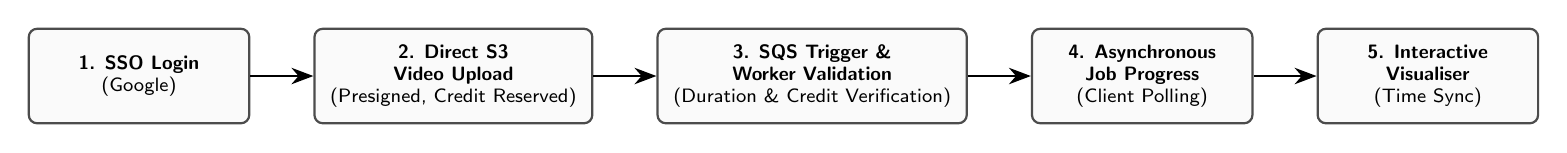
\begin{tikzpicture}[
        node distance=0.8cm,
        stepbox/.style={draw=black!70, thick, rounded corners=3pt, align=center, fill=black!2, inner sep=2mm, text=black, font=\sffamily\scriptsize, minimum width=2.8cm, minimum height=1.2cm},
        arrow/.style={-{Stealth[scale=1.2]}, thick, text=black!80}
    ]

    \node[stepbox] (s1) {\textbf{1. SSO Login}\\(Google)};
    \node[stepbox, right=of s1] (s2) {\textbf{2. Direct S3}\\\textbf{Video Upload}\\(Presigned, Credit Reserved)};
    \node[stepbox, right=of s2] (s3) {\textbf{3. SQS Trigger \&}\\\textbf{Worker Validation}\\(Duration \& Credit Verification)};
    \node[stepbox, right=of s3] (s4) {\textbf{4. Asynchronous}\\\textbf{Job Progress}\\(Client Polling)};
    \node[stepbox, right=of s4] (s5) {\textbf{5. Interactive}\\\textbf{Visualiser}\\(Time Sync)};

    \draw[arrow] (s1) -- (s2);
    \draw[arrow] (s2) -- (s3);
    \draw[arrow] (s3) -- (s4);
    \draw[arrow] (s4) -- (s5);

    \end{tikzpicture}%
    }
    \vspace{-2mm}
    \caption{NeuroLens End-to-End User Journey}
    \vspace{-4mm}
\end{figure}
\FloatBarrier

% ==========================================================================
% PAGE 3: Cloud SaaS Architecture
% ==========================================================================
\section*{\textsf{3. Cloud SaaS Architecture \& System Design}}

\begin{figure}[H]
\centering
\resizebox{\textwidth}{!}{%
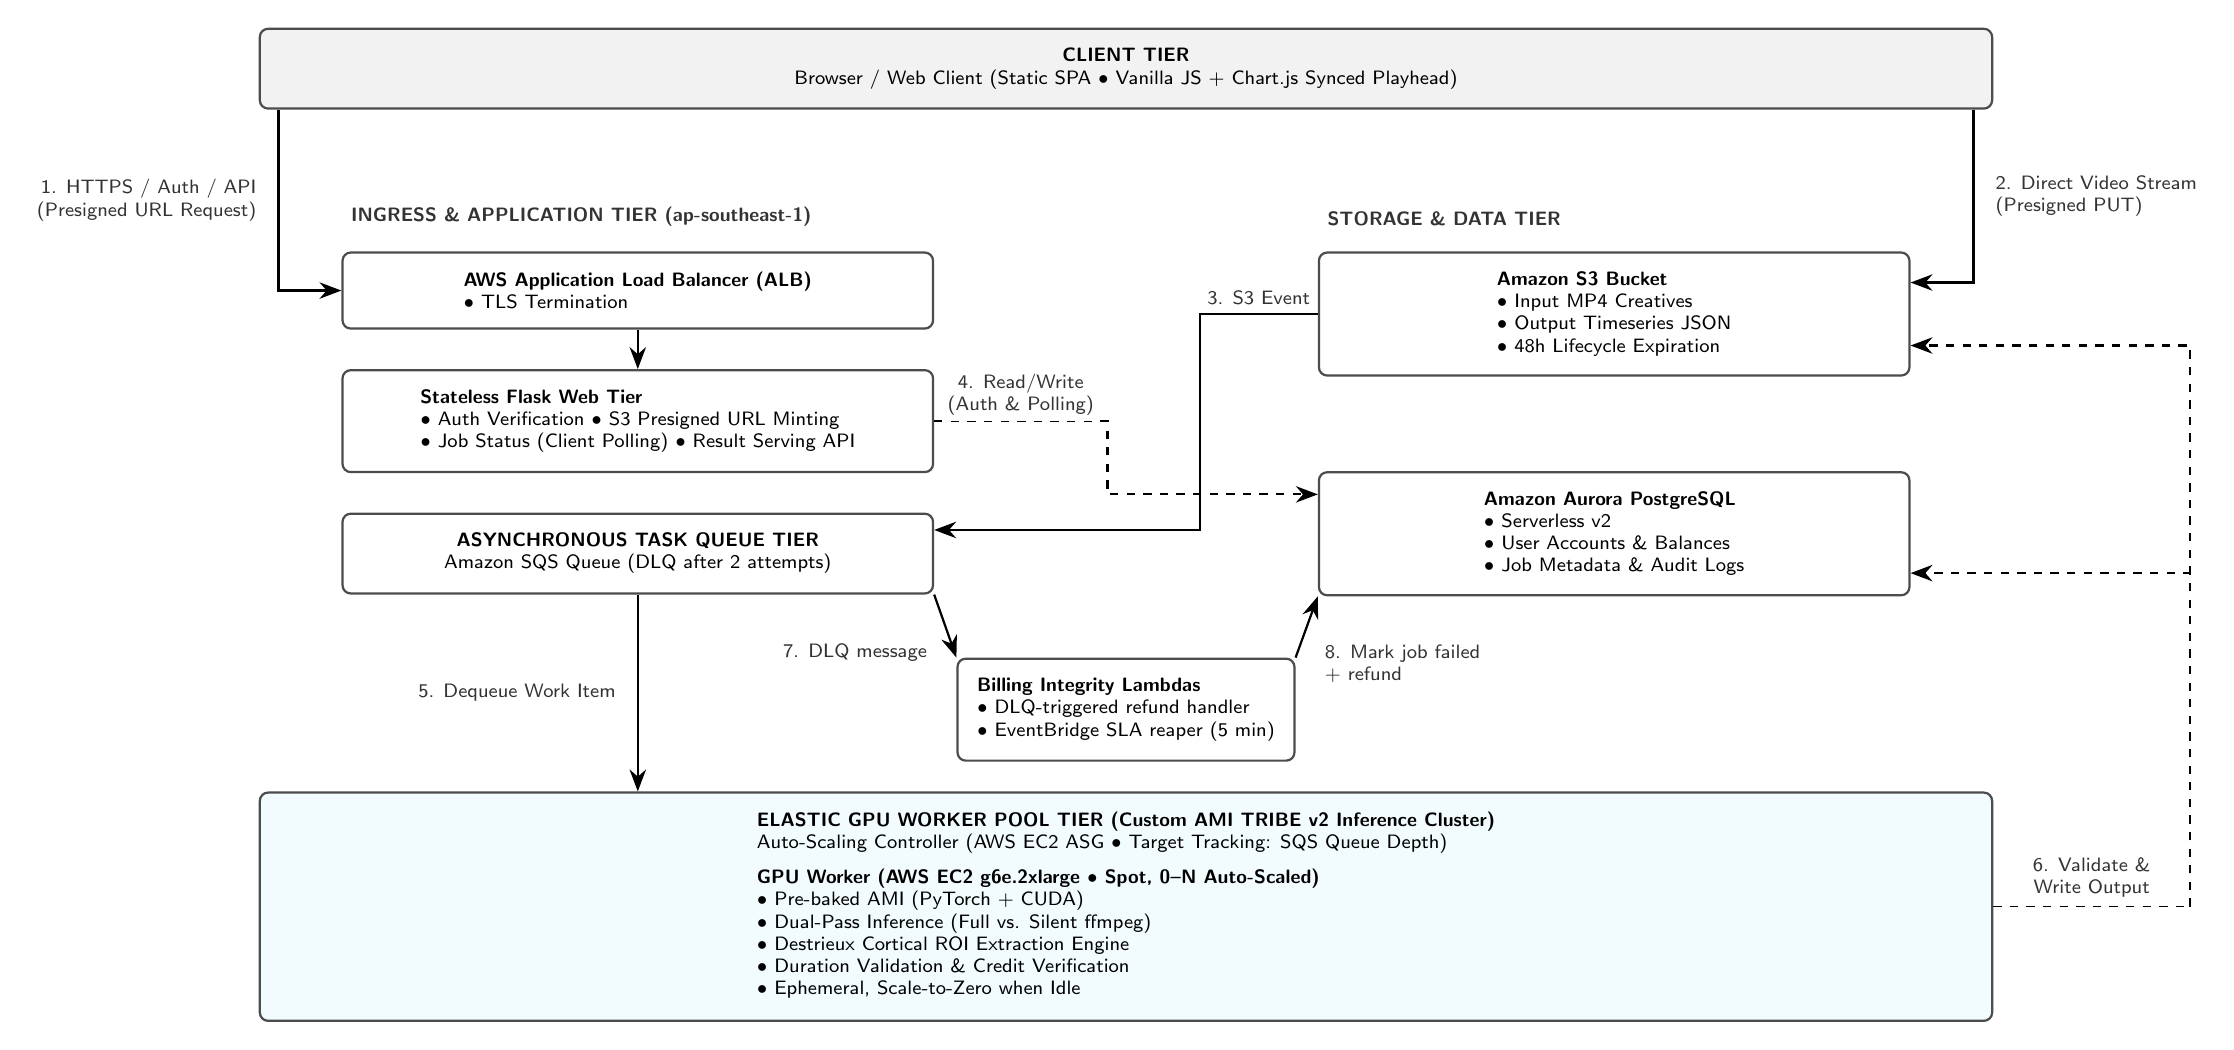
\begin{tikzpicture}[
    node distance=1.2cm and 1.8cm,
    box/.style={draw=black!70, thick, rounded corners=3pt, align=left, fill=white, inner sep=2.5mm, text=black, font=\sffamily\scriptsize},
    centerbox/.style={draw=black!70, thick, rounded corners=3pt, align=center, fill=white, inner sep=2.5mm, text=black, font=\sffamily\scriptsize},
    arrow/.style={-{Stealth[scale=1.2]}, thick, text=black!80, font=\sffamily\scriptsize}
]

% Client Tier (Expanded to 22cm to encapsulate the outer drop lines)
\node[centerbox, fill=black!5, minimum width=22cm] (client) {\textbf{CLIENT TIER}\\Browser / Web Client (Static SPA $\bullet$ Vanilla JS + Chart.js Synced Playhead)};

% App Tier Nodes (Left Column)
\node[box, below=1.8cm of client, xshift=-6.2cm, minimum width=7.5cm] (alb) {\textbf{AWS Application Load Balancer (ALB)}\\$\bullet$ TLS Termination};
\node[box, below=0.5cm of alb, minimum width=7.5cm] (flask) {\textbf{Stateless Flask Web Tier}\\$\bullet$ Auth Verification \hfill $\bullet$ S3 Presigned URL Minting\\$\bullet$ Job Status (Client Polling) \hfill $\bullet$ Result Serving API};
\node[centerbox, below=0.5cm of flask, minimum width=7.5cm] (sqs) {\textbf{ASYNCHRONOUS TASK QUEUE TIER}\\Amazon SQS Queue (DLQ after 2 attempts)};

% Explicitly anchored Application Tier Label
\node[above=2mm of alb.north west, anchor=south west, font=\sffamily\scriptsize\bfseries, text=black!80] {INGRESS \& APPLICATION TIER (ap-southeast-1)};

% Storage Tier Nodes (Right Column)
\node[box, below=1.8cm of client, xshift=6.2cm, minimum width=7.5cm] (s3) {\textbf{Amazon S3 Bucket}\\$\bullet$ Input MP4 Creatives\\$\bullet$ Output Timeseries JSON\\$\bullet$ 48h Lifecycle Expiration};
\node[box, below=1.2cm of s3, minimum width=7.5cm] (aurora) {\textbf{Amazon Aurora PostgreSQL}\\$\bullet$ Serverless v2\\$\bullet$ User Accounts \& Balances\\$\bullet$ Job Metadata \& Audit Logs};

% Explicitly anchored Storage Tier Label
\node[above=2mm of s3.north west, anchor=south west, font=\sffamily\scriptsize\bfseries, text=black!80] {STORAGE \& DATA TIER};

% NEW NODE: Billing Integrity Lambdas (positioned below and between SQS and Aurora to prevent overlap)
\node[box, below=0.8cm of sqs, xshift=6.2cm] (lambda) {\textbf{Billing Integrity Lambdas}\\$\bullet$ DLQ-triggered refund handler\\$\bullet$ EventBridge SLA reaper (5 min)};

% GPU Tier (Pushed down to accommodate the Lambda box)
\node[box, below=2.5cm of sqs, xshift=6.2cm, minimum width=22cm, fill=cyan!5] (gpu) {
    \textbf{ELASTIC GPU WORKER POOL TIER (Custom AMI TRIBE v2 Inference Cluster)}\\
    Auto-Scaling Controller (AWS EC2 ASG $\bullet$ Target Tracking: SQS Queue Depth)\\[1.5mm]
    \centering
    \begin{tabular}{@{}l@{}}
    \textbf{GPU Worker (AWS EC2 g6e.2xlarge $\bullet$ Spot, 0--N Auto-Scaled)} \\
    $\bullet$ Pre-baked AMI (PyTorch + CUDA) \\
    $\bullet$ Dual-Pass Inference (Full vs. Silent ffmpeg) \\
    $\bullet$ Destrieux Cortical ROI Extraction Engine \\
    $\bullet$ Duration Validation \& Credit Verification \\
    $\bullet$ Ephemeral, Scale-to-Zero when Idle
    \end{tabular}
};

% ================= Clean Top-Down Interactions =================

% Coordinates for exact vertical border alignment to prevent arrows from piercing wide nodes
\coordinate (s3_in)      at ($(s3.east) + (0, 4mm)$);
\coordinate (sqs_in)     at ($(sqs.east) + (0, 3mm)$);
\coordinate (aurora_in4) at ($(aurora.west) + (0, 5mm)$);
\coordinate (aurora_in6) at ($(aurora.east) + (0, -5mm)$);
\coordinate (s3_in6)     at ($(s3.east) + (0, -4mm)$);

% 1. Drop vertically from client to ALB
\draw[arrow] (client.south -| alb.west) ++(-0.8,0) coordinate (drop1) 
    -- node[left=1.5mm, align=right] {1. HTTPS / Auth / API\\(Presigned URL Request)} (drop1 |- alb.west) 
    -- (alb.west);

% 2. Drop vertically from client to S3
\draw[arrow] (client.south -| s3.east) ++(0.8,0) coordinate (drop2) 
    -- node[right=1.5mm, align=left] {2. Direct Video Stream\\(Presigned PUT)} (drop2 |- s3_in) 
    -- (s3_in);

% App internal flow
\draw[arrow] (alb.south) -- (flask.north);

% 3. S3 ObjectCreated Event to SQS
\draw[arrow] (s3.west) -- ++(-1.5,0) coordinate (drop3) -- (drop3 |- sqs_in) -- (sqs_in);
\path (s3.west) -- (drop3) node[midway, above, font=\sffamily\scriptsize, text=black!80] {3. S3 Event};

% 4. Read/Write for Auth & Polling
\draw[arrow, dashed] (flask.east) -- ++(2.2,0) coordinate (drop4) -- (drop4 |- aurora_in4) -- (aurora_in4);
\path (flask.east) -- (drop4) node[midway, above, align=center, font=\sffamily\scriptsize, text=black!80, fill=white, inner sep=2pt] {4. Read/Write\\(Auth \& Polling)};

% 5. Dequeue to GPU
\draw[arrow] (sqs.south) -- node[left=1.5mm] {5. Dequeue Work Item} (gpu.north -| sqs.south);

% 6. Read / Write Artifacts
\draw[dashed] (gpu.east) -- ++(2.5,0) coordinate (rt);
\draw[arrow, dashed] (rt) |- (aurora_in6);
\draw[arrow, dashed] (rt) |- (s3_in6);
\path (gpu.east) -- (rt) node[midway, above, align=center, font=\sffamily\scriptsize, text=black!80] {6. Validate \&\\Write Output};

% 7 & 8. DLQ to Lambda and Lambda to Aurora
\draw[arrow] (sqs.south east) -- node[below left=1mm and 1mm, align=right, font=\sffamily\scriptsize, text=black!80] {7. DLQ message\\} (lambda.north west);
\draw[arrow] (lambda.north east) -- node[below right=1mm and 1mm, align=left, font=\sffamily\scriptsize, text=black!80] {8. Mark job failed\\+ refund} (aurora.south west);

\end{tikzpicture}
}
\caption{NeuroLens Cloud SaaS Architecture and Data Flow}
\vspace{-1mm}
\end{figure}

Every design decision balances the need for elastic scalability with the engineering constraints of an early-stage business. We explicitly prioritised architectural simplicity, strict statelessness, and capital efficiency over premature enterprise optimisation:

\begin{itemize}
    \item \textbf{Ingestion (Separating Data vs. Control Planes):} To separate data and control planes, we routed the heavy video upload stream away from the API web tier: sending 50--250~MB ad creatives through Flask would saturate bandwidth and block concurrent sessions. The web tier instead acts only as an authenticator, minting a presigned S3 URL for direct client upload. To prevent the GPU worker fetching an incomplete file, SQS is triggered natively by the S3 \texttt{ObjectCreated} event rather than by Flask. Because this event lacks session context, Flask encodes the User ID into the S3 object key during minting for billing attribution.

    \item \textbf{Compute (Raw EC2 Spot vs. Managed Kubernetes/EKS):} TRIBE v2's $\sim$40~GB VRAM requirement rules out serverless options like AWS Lambda outright. We weighed raw EC2 Spot against managed Kubernetes (EKS)---which is the enterprise standard but adds steep control-plane costs ($\sim$\$73/month) and configuration overhead---and chose an EC2 Auto-Scaling Group on \texttt{g6e.2xlarge} Spot instances, cutting compute costs by $\sim$67\% versus On-Demand while scaling to zero when idle. The compute tier can later migrate to EKS for a hybrid On-Demand/Spot node group once enterprise SLAs require guaranteed processing times. Spot pricing floats with demand and carries a $\sim$2-minute interruption risk, absorbed via automatic requeueing rather than passed on to the user.

    \item \textbf{Cold-Start Mitigation (Hybrid AMIs vs. Runtime Docker Pulls):} Pulling a 20+~GB container image (PyTorch + CUDA + 5B parameter weights) during an ASG scale-out event introduces 5--8 minutes of latency. To mitigate this, instances boot directly from a custom Amazon Machine Image (AMI) with all heavy dependencies pre-baked. To avoid rebuilding a 30~GB AMI for every minor bug fix, a lightweight \texttt{UserData} script pulls the latest Python inference logic on boot. This approach trades the strict immutability of full containerisation for agile code updates and a cold-start latency meaningfully faster than the 5--8 minute container-pull baseline, to be measured empirically in Experiment~2.

    \item \textbf{State Tracking (Stateless Polling vs. WebSockets):} We deliberately kept the web tier strictly stateless. Tracking asynchronous GPU progress is handled via client-side long-polling (every 5 seconds) rather than persistent WebSockets or Server-Sent Events. Despite added DB read volume and minor UI latency, this lets the Application Load Balancer route traffic dynamically to any Flask node without requiring a costly Redis pub/sub broker to manage connection states. As concurrent volume grows and database read-thrashing becomes a concern, the system can migrate to a persistent WebSocket layer backed by Amazon ElastiCache.

    \item \textbf{Validation (Worker Consolidation vs. Microservice Sprawl):} Extracting video duration via \texttt{ffprobe} could theoretically run in an S3-triggered Lambda, but compiling \texttt{ffprobe} into a Lambda Layer is complex and brittle. We instead moved duration validation into the EC2 GPU worker, avoiding microservice sprawl. This introduces a ``denial-of-wallet'' vector where low-credit submissions could trigger billable GPU time. Client-side duration estimation and pre-upload credit checks keep most such requests off the GPU tier, with a CPU-only Fargate pre-processing queue as future work once volume demands it.

    \item \textbf{Billing Integrity (Reservation vs. Simple Debit):} A single debit-on-completion model would leave GPU spend uncapped if a user's balance ran out mid-job. Instead, a reservation is placed at upload, adjusted once the actual duration is verified, and captured on completion, with any unused amount released. Failure recovery is handled automatically by two small, event-driven functions that detect failed or stuck jobs and trigger the corresponding refund, so a lost job never means a silent loss to the user.

        \item \textbf{Payment Security (Hosted Checkout vs. Direct Card Handling):} Handling card data directly introduces meaningful information security risk and compliance burden. We therefore chose Stripe with its standard hosted Checkout flow, which keeps card data off NeuroLens's own servers entirely and qualifies the platform for the simplest PCI-DSS validation tier (SAQ-A), while still supporting the usage-based, credit-pack billing model described in Section 2.2.

    \item \textbf{Data Tier (ACID Transactions vs. NoSQL):} Financial ledger logic requires strict transactional consistency. DynamoDB's lower latency comes at the cost of complex \texttt{TransactWriteItems} logic for concurrent workflows. We chose Aurora PostgreSQL (Serverless v2) for native ACID guarantees and JSONB indexing, storing job metadata and billing records alongside an S3 pointer to the full result JSON. Serverless v2 auto-pauses at 0 ACUs during idle periods to reduce cost, and can be kept at a 0.5-ACU minimum for responsiveness. An atomic conditional status update ensures at most one worker can claim a queued job, preventing duplicate processing under SQS's at-least-once delivery. Credentials are managed via AWS Secrets Manager rather than application configuration.
\end{itemize}

% ==========================================================================
% PAGE 4: Implementation Roadmap
% ==========================================================================
\section*{\textsf{4. Implementation Roadmap}}

Four milestones deliver the NeuroLens cloud SaaS from initial infrastructure setup to a deployed, evaluated service:

\vspace{1mm}
\noindent
\begin{tabularx}{\textwidth}{|l|l|X|}
\hline
\rowcolor{black!5}
\textbf{Milestone} & \textbf{Dates} & \textbf{Core Technical Focus \& Deliverables} \\
\hline
\textbf{M1} & \textbf{29 Sept -- 8 Oct} & \textbf{Cloud Storage \& Task Queue Decoupling:}
\begin{itemize}[leftmargin=*, itemsep=3pt, topsep=3pt, parsep=1pt]
    \item S3 presigned URL generation with size/MIME-type validation; direct client-side upload.
    \item Amazon SQS worker process decoupled from the synchronous Flask handler.
    \item Minimal upload UI: file picker with client-side duration read and estimated-cost display before upload.
\end{itemize} \\
\hline
\textbf{M2} & \textbf{9 -- 19 Oct} & \textbf{GPU AMI Provisioning \& Elastic Autoscaling:}
\begin{itemize}[leftmargin=*, itemsep=3pt, topsep=3pt, parsep=1pt]
    \item Custom AMI (PyTorch + CUDA 12.4 + TRIBE v2 weights pre-baked) deployed via EC2 Auto Scaling Group, with UserData pulling the latest inference code on boot.
    \item EC2 ASG configured with CloudWatch SQS queue-depth scaling.
    \item Begin latency and Locust load-test data collection (Experiments 1 \& 2).
    \item Job progress UI: client-side polling view for queue and processing status.
\end{itemize} \\
\hline
\textbf{M3} & \textbf{20 -- 30 Oct} & \textbf{Authentication, Billing \& Result Persistence:}
\begin{itemize}[leftmargin=*, itemsep=3pt, topsep=3pt, parsep=1pt]
    \item Google OAuth2 SSO and PostgreSQL schema for user accounts and credit balances.
    \item Credit debiting engine, job history, and CSV result export.
    \item Begin cloud vs.\ on-premise TCO benchmark runs (Experiment 3).
    \item Google SSO login screen, credit balance/job history dashboard, and Chart.js synced-playhead visualiser.
\end{itemize} \\
\hline
\textbf{M4} & \textbf{31 Oct -- 13 Nov} & \textbf{Usability Evaluation \& Analysis:}
\begin{itemize}[leftmargin=*, itemsep=3pt, topsep=3pt, parsep=1pt]
    \item 5-participant SUS usability study with task performance metrics.
    \item Consolidation and analysis of all benchmark results for the Final Report.
\end{itemize} \\
\hline
\end{tabularx}

% ==========================================================================
% PAGE 5: Evaluation \& References
% ==========================================================================
\section*{\textsf{5. Plan for Evaluation}}
We plan three technical experiments to validate system performance and cloud economics, and a structured usability study with five participants. While this evaluation plan is designed to thoroughly validate system performance and usability, verifying the predictive fidelity of TRIBE v2's outputs against real-world ad performance is out of scope for this phase due to data availability, and is noted as future work.

\subsection*{\textsf{5.1 System Evaluation Plan (Technical \& Economic Benchmarks)}}
\begin{enumerate}
    \item \textbf{Experiment 1 --- End-to-End Latency Breakdown:} Measure per-stage duration (Upload $\rightarrow$ Queue Wait $\rightarrow$ Dual Inference $\rightarrow$ ROI Extraction $\rightarrow$ Client Render) across 15s, 30s, and 60s video lengths. Inference duration and peak VRAM are logged automatically by the pipeline.
    \item \textbf{Experiment 2 --- Elastic Scaling \& Throughput Under Load:} Using Locust, simulate concurrent submission bursts (1, 5, 10, 20 jobs) in two stages: lower bursts (1, 5) measure GPU cold-start latency and per-worker throughput as the worker pool scales with demand; higher bursts (10, 20) confirm the queue absorbs backlog gracefully once autoscaling capacity is saturated, with a full drain once load subsides. A Spot interruption will be manually injected to validate the SQS requeue mechanism.
    \item \textbf{Experiment 3 --- Cloud vs.\ On-Premise TCO Benchmark:} Execute 10--15 benchmark runs per video duration (15s, 30s, 60s) on cloud Spot instances and available team hardware ($\sim$60--90 runs total). Power consumption is modelled from published hardware thermal design power (TDP) and measured inference durations. Results use measured inference runtimes to estimate cloud and on-premise costs, then compare those estimates with the Section 2.2 breakeven point.
\end{enumerate}

\subsection*{\textsf{5.2 User Evaluation Plan (SaaS Usability \& Qualitative Feedback)}}
\begin{itemize}
    \item \textbf{Participant Cohort (N=5):} Following Nielsen's finding that five participants uncover approximately 85\% of usability issues in formative testing (Nielsen, 2000), we recruit 5 users from the target demographic --- student content creators and peers managing digital media channels. Participants will provide informed consent covering upload of self-selected ad samples.
    \item \textbf{End-to-End Creative Audit Scenario:} Participants complete one end-to-end workflow: uploading an ad creative, observing real-time cloud processing progress, and exploring the synchronised playhead timeline to identify attention peaks and drop-off moments.
    \item \textbf{Evaluation Metrics \& Qualitative Feedback:}
    \begin{itemize}
        \item \textit{System Usability Scale (SUS; Brooke, 1996):} Standardised 10-item questionnaire targeting the Grade A threshold ($\ge$80/100); scores below 80 will inform targeted future UI refinements.
        \item \textit{Task Performance:} Task success rate and time-on-task for the core creative audit workflow.
        \item \textit{Structured Qualitative Feedback:} Open-ended evaluation capturing (1) dashboard clarity and playhead responsiveness, (2) comprehension of cortical ROI labels, and (3) perceived commercial value of the \$0.90/ad pricing model.
    \end{itemize}
\end{itemize}

\section*{\textsf{6. Conclusion}}
NeuroLens targets a market that current tools underserve, delivering cloud-native cortical video analysis as a credit-pack and subscription-based service. Every architectural choice is driven by a concrete constraint: Spot GPU workers for elastic compute economics, SQS queue decoupling for fault-tolerant async processing, Aurora PostgreSQL for ACID credit integrity, and presigned S3 ingestion to keep the web tier stateless.

The unit economics in Section 2.2 demonstrate that elastic cloud hosting remains cost-effective below approximately 1,475 videos/month, eliminating prohibitive hardware CAPEX for target users while scaling efficiently to zero during idle periods. Overall, the architecture provides a robust, fault-tolerant foundation for scalable video engagement prediction, with empirical performance and usability evaluations scheduled across the upcoming milestone phases.

\vspace{1mm}
\begin{tcolorbox}[colback=black!2, colframe=black!15, arc=3pt, boxrule=0.5pt, left=6pt, right=6pt, top=4pt, bottom=4pt]
{\footnotesize \textbf{AI Declaration:} AI tools were used to assist in refining the prose, as a thought partner to evaluate the cloud architectural trade-offs in Section 3, and to help structure the evaluation plan in Section 5. This process deepened the team's practical understanding of both cloud-native system design and robust testing methodologies. However, all final technical design decisions, cost analyses, and evaluation methodologies were ultimately determined and validated by the project team.}
\end{tcolorbox}

\section*{\textsf{References}}
\begin{multicols}{2}
\scriptsize
\noindent
\textbf{1. Allison, T., et al.} (2000). Social perception from visual cues: role of the STS. \textit{Trends Cogn Sci}, 4(7), 267--278.\\
\textbf{2. Armbrust, M., et al.} (2010). A view of cloud computing. \textit{Commun ACM}, 53(4), 50--58.\\
\textbf{3. Binder, J. R., et al.} (2000). Human temporal lobe activation by speech and nonspeech sounds. \textit{Cereb Cortex}, 10(5), 512--528.\\
\textbf{4. Brooke, J.} (1996). SUS: A `quick and dirty' usability scale. \textit{Usability Eval Ind}, 189--194.\\
\textbf{5. d'Ascoli, S., et al.} (2026). TRIBE v2: Trimodal Brain Encoder. \textit{Meta FAIR Open Research}.\\
\textbf{6. Destrieux, C., et al.} (2010). Parcellation of human cortical gyri and sulci. \textit{NeuroImage}, 53(1), 1--15.\\
\textbf{7. Downing, P. E., et al.} (2001). A cortical area specialized for body perception. \textit{Science}, 293(5539), 2470--2473.\\
\textbf{8. Epstein, R., \& Kanwisher, N.} (1998). Cortical representation of visual environment. \textit{Nature}, 392(6676), 598--601.\\
\textbf{9. Frith, C. D., \& Frith, U.} (2006). Neural basis of social interaction. \textit{Lancet}, 367(9523), 1699--1708.\\
\textbf{10. Kanwisher, N., et al.} (1997). The fusiform face area in face perception. \textit{J Neurosci}, 17(11), 4302--4311.\\
\textbf{11. Nielsen, J.} (2000). \textit{Why You Only Need to Test with 5 Users}. Nielsen Norman Group, Alertbox.\\
\textbf{12. Venkatraman, V., et al.} (2015). Predicting advertising success beyond traditional measures. \textit{J Mark Res}, 52(4), 436--452.
\end{multicols}

\end{document}